\section{Описание прототипа}\label{prototype}

В описании к авторскому свидетельству №844986, кл. G 01 B 7/06 (по заявке №4822394/28 от 22.03.90 г., автор В.Г.Панов) представлено устройство \glqq Емкостной датчик микроперемещений\grqq, функциональная схема которого приведена на рисунке~\ref{schema}.

\begin{figure}[h]
	\centering
	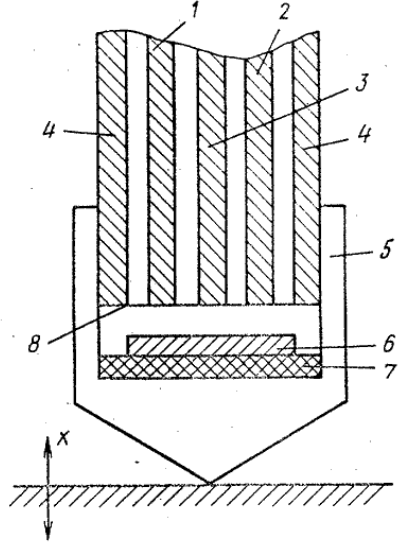
\includegraphics[width=0.4\textwidth]{schema.png}
	\caption{Функциональная схема датчика}
	\label{schema}
\end{figure}

Датчик содержит неподвижные потенциальный $1$ и измерительный $2$ электроды и охватывающие их внутренний $3$ и внешний $4$ экраны. Торцы электродов и экранов лежат в рабочей плоскости датчика. Снаружи боковой цилиндрической поверхности внешнего экрана $4$ размещен с возможностью возвратно- поступательного движения щуп $5$, во внутренней полости которого размещена металлическая пластина $6$, которая электрически изолирована от корпуса датчика и расположена параллельно рабочей плоскости его электродов и экранов. При перемещении щупа $5$ изменяется зазор между пластиной $6$ и рабочими торцами электродов и экранов, что приводит к изменению емкости датчика.

Датчик работает следующим образом: при перемещении объекта изменяется воздушный зазор между плоскостью металлической пластинки $5$ и рабочей плоскостью $8$ 
электродов $1$ и $2$ и экранов $3$ и $4$ датчика, вследствие чего изменяется выходное напряжение $U_{\text{вых}}$, снимаемое с измерительного электрода $2$ датчика. Чувствительность датчика зависит от величины диэлектрической постоянной материала контролируемого объекта и максимальна в диапазоне $0 - x_{\text{мин}}$, где $x_{\text{мин}}$~-- величина микроперемещения, когда металлическая пластина $6$ не заземлена. Герметизация щупа $5$ позволяет свести к минимуму погрешности, связанные с влиянием внешних условий.


\begin{figure}[h]
	\centering
	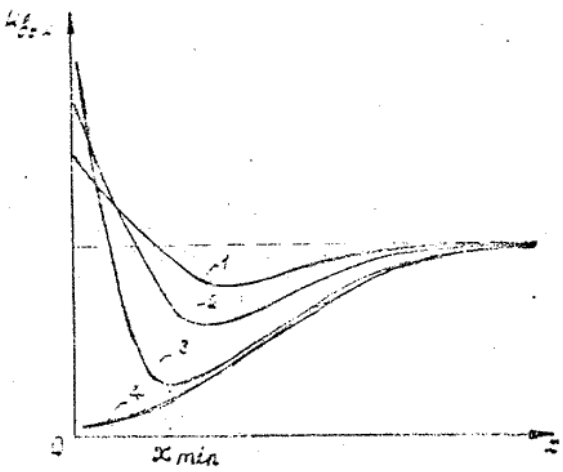
\includegraphics[width=0.4\textwidth]{out.png}
	\caption{Выходная характеристика в зависимости от диэлектрической проницаемости}
	\label{out}
\end{figure}


\section{Анализ и синтез по закону полноты частей системы}

%рабочий орган -- величина емкости между электродами и пластиной.
%трансмиссия -- пластина 6, подложка 7.
%двигатель -- щуп 7.

Определим основные части системы, представленной на рисунке~\ref{schema}. Сначала, определим рабочий орган -- Ро. Датчик предназначен для измерения расстояния. Расстояние выражается в изменении емкости между рабочей плоскостью 8 и пластиной 6. Изменение емкости влияет на выходное напряжение, которое измеряется при помощи с "конденсатора", образованного следующими элементами потенциальным электродом 1, пластиной 6 и измерительным электродом 2. 

Далее определим двигатель как часть системы, вырабатывающей энергетику. Здесь двигателем является балка, в которую упирается щуп 5. Тогда трансмиссией являются щуп, подложка 7 и пластина 6. Органов управления в рассматриваемом датчике нет, поэтому система является неполной. Структурная схема представлена на рисунке~\ref{first_sys}

\begin{figure}[h]
	\centering
	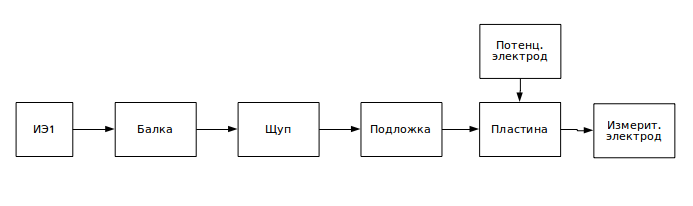
\includegraphics[width=1\textwidth]{pic0.png}
	\caption{Структурная схема рассматриваемой системы}
	\label{first_sys}
\end{figure}

Чтобы получить новые технические решения с использованием закона полноты частей  системы, можно добавить недостающие элементы в систему. 

Каждая ТС должна включать четыре части: двигатель, трансмиссию, рабочий орган и орган управления. Для синтеза ТС необходимо наличие этих четырех частей и их минимальная пригодность к выполнению функций системы.

Добавим в систему орган управления (ОУ).

Добавим в систему измерительную часть -- мостовую схему измерения, представленную на рисунке~\ref{im:bridge}, где $C_x$~-- представление датчика, как переменный конденсатор, $R_1$ и $R_2$~-- резисторы, У~-- усилитель, ИБ~-- измерительный прибор. Переменный конденсатор $C_3$, при помощи которого сможем подстраивать нулевое положения датчика. Этот конденсатор будет выступать в качестве Органа управления.


\begin{figure}[h]
	\centering
	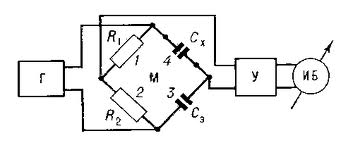
\includegraphics[width=0.6\textwidth]{bridge.jpg}
	\caption{Схема измерения емкости датчика с подстройкой}
	\label{im:bridge}
\end{figure}


\begin{figure}[h!]
	\centering
	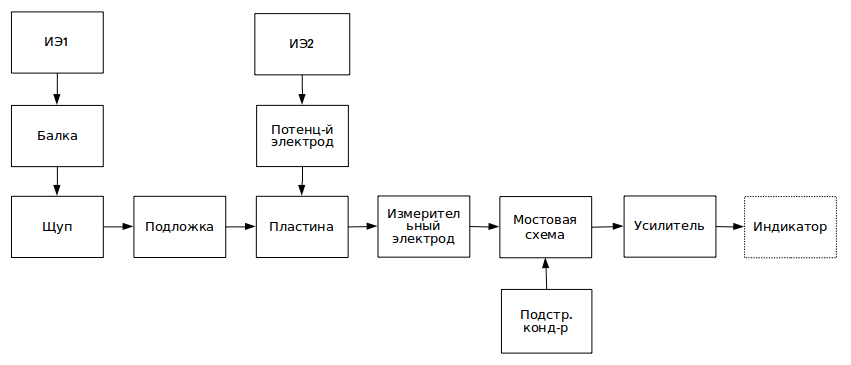
\includegraphics[width=1\textwidth]{pic1.png}
	\caption{Структурная схема полной системы}
	\label{pic1}
\end{figure}

Чтобы получить новые технические решения с использованием закона полноты частей системы, можно использовать линию на вытеснение человека из ТС. В соответствии с
линией вытеснения действия человека необходимо искать на окончании этой линии -- в органах управления.

В рассматриваемой системе балка давит на щуп, который в свою очередь это давление передает через подложку 7 на пластину 6. Пластина шесть изменяет свое положение относительно плоскости электродов 8. Электроды и пластина, образующие конденсатор, емкость которого изменяется, в результате чего с измерительной схемы на усилитель передается отклонение пластины от нулевого положения, заданного человеком при помощи подстроечного конденсатора. Для вытеснения этой функции человека этот конденсатор должен подстраиваться автоматически при включении системы. Нужно заменить конденсатор на устройство подстройки емкости, при помощи подачи некоторого информационного сигнала 
с надсистемы.

Система получается с автоматической калибровкой. Такая система обладает меньшими ошибками и более простой в использовании. 

Таким образом, с точки зрения закона получили полную систему.


\subsection{Анализ и синтез по закону энергетической и информационной проводимости ТС}


Необходимым условием принципиальной жизнеспособности ТС является сквозной проход энергии и информации по всем частям технической системы. 

Проанализируем систему с рисунка~\ref{pic1} по закону энергетической проводимости. Построение линии начнем с ИП, рисунок~\ref{im:bridge}, он выделяет электрическую энергию. Электрическое поле ИП воздействие на потенциальный электрод, на выходе которого формируется напряжение. Информативный параметр электрического поля в данном случае -- это переменное напряжения. 
Поле давления действует на щуп, в результате чего он изменяет свое положение относительно корпуса. 
Поле давления от щупа воздействует на подложке. Поле давления от подложки воздействует на пластину. Электрическое поле от потенциального электрода воздействует на пластину. Электрическое поле от пластины воздействует на измерительный электрод. Электрическое поле от Измерительного электрода воздействует на Мостовую измерительную схему. Информационным параметр электрического поля в этом случае -- это рассогласование емкости эталонного конденсатора и емкости между электродами и пластиной. Поле электрического поля от мостовая схемы воздействует на усилитель. Выходным информационным параметром усилителя будет напряжение.


\begin{figure}[h!]
	\centering
	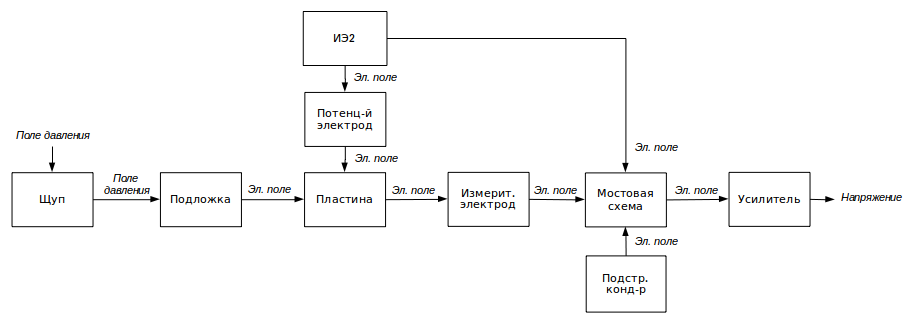
\includegraphics[width=1\textwidth]{pic2.png}
	\caption{Линия прохода энергии и информации}
	\label{}
\end{figure}

Для синтеза новых решений можно замкнуть линию прохождения энергии, получив кольцо. 

По этому закону можно дополнить систему на входе регулятором и пьезодвигателем, поле давление которого будет воздействовать на щуп. Для этого выход усилителя замкнем на вход регулятора, напряжение которого будем подавать на пьезодвигатель.

\begin{figure}[h!]
	\centering
	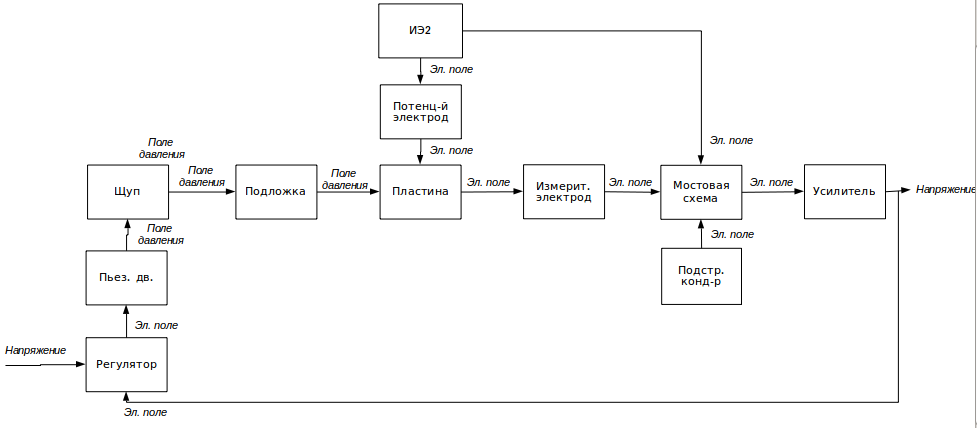
\includegraphics[width=1\textwidth]{pic3.png}
	\caption{Линия прохода энергии и информации с замкнутой схеме}
	\label{sogl}
\end{figure}

\section{Закон согласования-рассогласования технических систем}

Составляющие техническую систему части должны быть согласованы или, наоборот, рассогласованы между собой.

С точки зрения этого закона можно проверить согласованность по темпам протекания процессов, происходящих в основных частях системы.

Система рассогласована по темпам протекания процессов. Изменение расстояния между пластиной и плоскостью электродов, происходит медленнее, чем протекают токи в электрических схемах мостовой схемы и усилителя. Чтобы согласовать ее, можно заменить электрическую часть механической, в которой перемещение щупа через механические передачи будет преобразовываться в показания стрелочного индикатора.

С точки зрения энергетических параметром, полученная система на рисунке~\real{sogl} согласована по входным и выходным информационным сигналам.

Система рассогласована в части параметров материалов. Для согласования системы, чтобы избавиться от вредного явления трения между корпусом и щупом, а в перспективе и износа щупа, можно убрать щуп.

Рисунок с механическим измерением

\section{Анализ и синтез систем по закону увеличения степени идеальности}

Закон увеличения степени идеальности является одним из основных законом развития ТС. Под увеличением степени идеальности И в ТРИЗ понимается рост отношения суммы выполняемых системой полезных функций Фп к сумме факторов расплаты Фр.



%Для повышения степени идеальности путем увеличения числителя формулы необходимо возложить на систему еще одну или несколько функций, ранее ею не выполнявшихся. Например, при добавлении обратной связи, позволяющей стабилизировать конструкцию в зависимости от выходного напряжения можно получить новое устройство - стабилизирующая платформа. Факторами расплаты в этом случае будут являться добавление новых элементов в систему, таких как двигатель и редуктор.

%При добавлении датчиков, сигнализирующих о достижении крайнего положения отклонения, например герконов, получим еще одну функцию системы – контроль достижения предельного отклонения.

%Рисунок 6 – Использование датчиков крайнего положения

%Попробуем уменьшить знаменатель. Для этого исключим из системы какую-либо её часть, например элемент масштабирования. Измерение отклонения проводить по прежнему можно, но это уменьшит точность.

\section{Закон неравномерного развития технических систем}

%;ехнической системы появляются противоречия, происходит накопление и обострение противоречий.

%Выберем содержательную характеристику, которую будем улучшать.

%Для данного датчика выберем повышение чувствительности. Если отклонить конструкцию на очень малый угол, то на выходе катушек 4, 6 индуктивности не появляется напряжение, достаточное для формирования выходного сигнала.

%Чем тяжелее маятник, тем точнее будет измерение. Но увеличивается размер и тем самым деформируется шарнир. Возникает противоречие: маятник должен быть большим для увеличения точности и не большим, чтобы он не деформировал шарнир.

%Разрешим это противоречие с помощью алгоритма решения изобретательских задач (АРИЗ).

\newpage